\documentclass[11pt,a4paper]{article}
\usepackage[margin=1in]{geometry}
\usepackage{graphicx}
\usepackage{float}
\usepackage{amsmath}
\usepackage{hyperref}
\usepackage{array}
\usepackage{booktabs}
\usepackage{xcolor}
\graphicspath{{./report_assets/}{./image/}}
\hypersetup{hidelinks}

\title{Homework 4 Report\\Markov Decision Process}
\author{Intelligent Robotics}
\date{April 17, 2026}

\begin{document}

\maketitle

\section{Overview}

Homework 4 contains two parts:

\begin{enumerate}
    \item Theoretical analysis for two small grid-world MDPs.
    \item Programming implementation of policy evaluation, policy iteration, and value iteration on the provided $20 \times 20$ map.
\end{enumerate}

The main implementation files for the programming part are:

\begin{itemize}
    \item \texttt{source/mdp.py}
    \item \texttt{source/grid\_map.py}
    \item \texttt{source/question1\_run.py}
    \item \texttt{source/question2\_run.py}
    \item \texttt{source/question3\_run.py}
\end{itemize}

\section{Part I: Theoretical Analysis}

\subsection{MDP Formulation}

For both theoretical cases, the grid world is modeled as an MDP with:

\begin{itemize}
    \item state set: the grid cells,
    \item action set: \{up, down, left, right\},
    \item transition model: deterministic motion with boundary clipping,
    \item reward: determined by the target cell and the case-specific rule.
\end{itemize}

The PDF statement does not explicitly give $\gamma$, so this report follows the usual lecture convention $\gamma = 1$ for the theoretical part. The goal cell $O$ is treated as a terminal state with value $0$.

\subsection{Case 1}

Case 1 uses a $3 \times 3$ grid with goal $O$ at the top-right cell and step reward $-1$ for every non-goal move.

The Bellman optimality equation is:
\[
V^*(s) = \max_a \left[ r(s,a,s') + V^*(s') \right].
\]

Both value iteration and policy iteration converge to the same optimal values:

\[
\begin{bmatrix}
-1 & 0 & 0 \\
-2 & -1 & 0 \\
-3 & -2 & -1
\end{bmatrix}
\]

An optimal policy is:

\begin{center}
\begin{tabular}{ccc}
\texttt{R} & \texttt{R} & \texttt{G} \\
\texttt{U/R} & \texttt{U/R} & \texttt{U} \\
\texttt{U/R} & \texttt{U/R} & \texttt{U}
\end{tabular}
\end{center}

The result is intuitive: the optimal action is always the shortest move toward the goal, and ties appear when moving up or right is equally good.

\subsection{Case 2}

Case 2 uses the same $3 \times 3$ grid with:

\begin{itemize}
    \item goal $O$ at the top-right cell,
    \item obstacle $B$ at the center cell,
    \item reward $0$ for entering $O$,
    \item reward $-1$ for entering $B$,
    \item reward $-0.1$ for all other non-goal moves.
\end{itemize}

Both value iteration and policy iteration converge to:

\[
\begin{bmatrix}
-0.1 & 0.0 & 0.0 \\
-0.2 & -0.1 & 0.0 \\
-0.3 & -0.2 & -0.1
\end{bmatrix}
\]

One optimal policy is:

\begin{center}
\begin{tabular}{ccc}
\texttt{R} & \texttt{R} & \texttt{G} \\
\texttt{U} & \texttt{U/R} & \texttt{U} \\
\texttt{U/R} & \texttt{R} & \texttt{U}
\end{tabular}
\end{center}

Compared with Case 1, the step cost is much smaller, so the value landscape is flatter. The policy still prefers short paths to the goal, while avoiding repeated visits to the obstacle cell because entering $B$ gives reward $-1$.

\subsection{Remark on the ``Equal Probability'' Phrase}

The homework text says that each action has equal probability. This can be interpreted in two different ways:

\begin{itemize}
    \item as the initial random policy before policy improvement,
    \item or as a fixed stochastic policy to be evaluated.
\end{itemize}

This report uses the first interpretation for the main answer because the question explicitly asks for both value iteration and policy iteration, which are optimal-control algorithms. The alternative fixed-policy values are recorded in \texttt{SUBMISSION.md} for reference.

\section{Part II: Programming}

\subsection{Implementation Summary}

The programming part required completing the core MDP algorithms in \texttt{source/mdp.py}. The following logic was implemented:

\begin{itemize}
    \item Bellman expectation update for policy evaluation,
    \item greedy action improvement for policy iteration,
    \item Bellman optimality update for value iteration,
    \item action extraction from the final value function,
    \item terminal-state handling for the goal state.
\end{itemize}

In \texttt{source/grid\_map.py}, the step function was also adjusted so that going out of bounds incurs a penalty but does not terminate the episode. This is important because otherwise the planner can incorrectly prefer ``crashing'' into the boundary instead of reaching the true goal.

\begin{figure}[H]
\centering
\includegraphics[width=0.48\textwidth]{mdp.png}
\caption{Provided $20 \times 20$ MDP map}
\end{figure}

\subsection{Question 1: Policy Evaluation}

Question 1 evaluates the initial uniform policy over the provided map. The iterative update is:
\[
V_{k+1}(s) = \sum_a \pi(a|s) \left[ r(s,a,s') + \gamma V_k(s') \right].
\]

Using the implemented solver with $\gamma = 0.95$ from the homework scaffold, the converged statistics are listed in Table~\ref{tab:q1-stats}.

\begin{table}[H]
\centering
\begin{tabular}{@{}ll@{}}
\toprule
Metric & Value \\
\midrule
Start-state value & $-38.8338$ \\
Goal-state value & $0.0$ \\
Minimum state value & $-69.5453$ \\
Maximum state value & $0.0$ \\
\bottomrule
\end{tabular}
\caption{Question 1 policy-evaluation statistics}
\label{tab:q1-stats}
\end{table}

\begin{figure}[H]
\centering
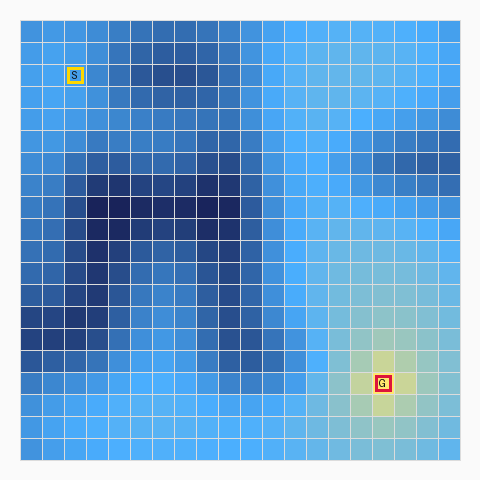
\includegraphics[width=0.78\textwidth]{q1_policy_evaluation_heatmap.png}
\caption{Policy-evaluation heatmap under the initial uniform policy}
\end{figure}

The heatmap shows that states trapped behind obstacle regions or far from the goal accumulate much lower expected return under the random initial policy.

\subsection{Question 2: Policy Iteration}

Question 2 alternates between policy evaluation and greedy policy improvement:
\[
\pi_{k+1}(s) = \arg\max_a \left[ r(s,a,s') + \gamma V^{\pi_k}(s') \right].
\]

The implemented policy iteration converged after $16$ improvement rounds. The final path from the start state $(2,2)$ reaches the goal $(16,16)$ in $28$ steps.

\begin{table}[H]
\centering
\begin{tabular}{@{}ll@{}}
\toprule
Metric & Value \\
\midrule
Policy-improvement rounds & 16 \\
Start-state value & $-12.4897$ \\
Steps to goal & 28 \\
Terminal state & $(16,16)$ \\
Final reward & $10.0$ \\
\bottomrule
\end{tabular}
\caption{Question 2 policy-iteration statistics}
\end{table}

\begin{figure}[H]
\centering
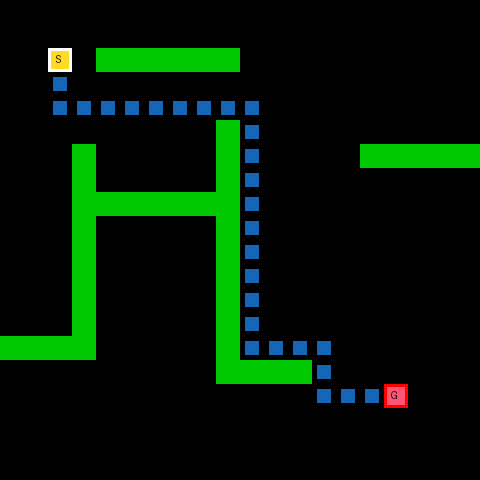
\includegraphics[width=0.78\textwidth]{q2_policy_iteration_path.png}
\caption{Final path produced by policy iteration}
\end{figure}

\subsection{Question 3: Value Iteration}

Question 3 uses value iteration:
\[
V_{k+1}(s) = \max_a \left[ r(s,a,s') + \gamma V_k(s') \right].
\]

According to the provided homework scaffold, the grid map for Question 3 uses \texttt{state\_prob = 0.8}. With that setting, value iteration converged after $26$ update rounds. The extracted greedy path again reaches $(16,16)$ in $28$ steps.

\begin{table}[H]
\centering
\begin{tabular}{@{}ll@{}}
\toprule
Metric & Value \\
\midrule
Value-iteration rounds & 26 \\
Start-state value & $-3.3307$ \\
Steps to goal & 28 \\
Terminal state & $(16,16)$ \\
Final reward & $10.0$ \\
\bottomrule
\end{tabular}
\caption{Question 3 value-iteration statistics}
\end{table}

\begin{figure}[H]
\centering
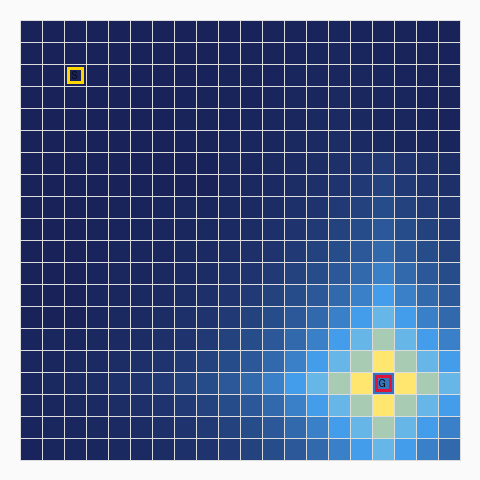
\includegraphics[width=0.78\textwidth]{q3_value_iteration_heatmap.png}
\caption{Value-iteration heatmap}
\end{figure}

\begin{figure}[H]
\centering
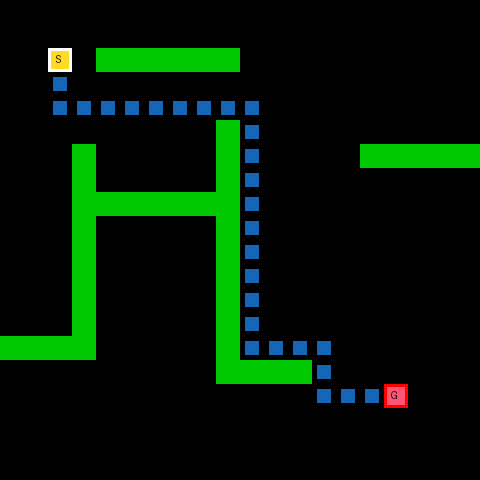
\includegraphics[width=0.78\textwidth]{q3_value_iteration_path.png}
\caption{Greedy path extracted from the value-iteration result}
\end{figure}

\subsection{Verification}

For reproducibility, a headless checker \texttt{source/verify\_hw4.py} was added. Running it prints:

\begin{itemize}
    \item Question 1 policy-evaluation statistics,
    \item Question 2 convergence rounds and final path,
    \item Question 3 convergence rounds and final path.
\end{itemize}

The verified policy-iteration and value-iteration paths are identical:

\begin{verbatim}
(2,2) -> (3,2) -> (4,2) -> (4,3) -> (4,4) -> (4,5) -> (4,6)
-> (4,7) -> (4,8) -> (4,9) -> (4,10) -> (5,10) -> (6,10)
-> (7,10) -> (8,10) -> (9,10) -> (10,10) -> (11,10)
-> (12,10) -> (13,10) -> (14,10) -> (14,11) -> (14,12)
-> (14,13) -> (15,13) -> (16,13) -> (16,14) -> (16,15)
-> (16,16)
\end{verbatim}

\section{How To Run}

Run from \texttt{hw4/source}:

\begin{verbatim}
python question1_run.py
python verify_hw4.py
\end{verbatim}

To run the original animated scripts for Questions 2 and 3:

\begin{verbatim}
pip install ir_sim==1.1.8 matplotlib
python question2_run.py
python question3_run.py
\end{verbatim}

To rebuild the report from the \texttt{hw4} directory:

\begin{verbatim}
python generate_report_assets.py
pdflatex report.tex
\end{verbatim}

\section{Conclusion}

The homework is completed in both theory and programming aspects. In the theoretical part, policy iteration and value iteration converge to the same optimal solution for both small MDP cases. In the programming part, the implemented algorithms correctly evaluate the initial policy, improve the policy to optimality, and compute the optimal value function on the provided map. The final policy-iteration and value-iteration solvers both reach the goal successfully with a $28$-step path.

\end{document}
